\documentclass{article}
\usepackage{amsmath,amssymb,amsfonts,amsthm, dsfont, color}
\usepackage{amsfonts}
\usepackage{tikz}
\usetikzlibrary{external}
\usetikzlibrary{shapes.misc, positioning}
\usetikzlibrary{decorations.pathreplacing}
\usetikzlibrary{arrows.meta, shapes,patterns.meta}

\tikzset{
  block/.style    = {draw, thick, rectangle, minimum width = 2em},
sblock/.style      = {draw, thick, rectangle, minimum height = 2em,
minimum width = 2em}, 
}
        
\definecolor{embed}{HTML}{AEF78E}
\definecolor{attn}{HTML}{f9e3ae}
\definecolor{ff}{HTML}{90F3FF}
\definecolor{lin}{HTML}{E15CEC}
\definecolor{mask1}{HTML}{4D4847}
\definecolor{mask2}{HTML}{30343F}

\newcommand{\vect}[1]{\boldsymbol{#1}}
\newcommand{\bx}{\vect{x}}
\newcommand{\by}{\vect{y}}
\newcommand{\bz}{\vect{z}}
\newcommand{\logit}{\mathrm{logit}}
\newcommand{\btheta}{\vect{\theta}}
\newcommand{\thetabar}{\bar{\btheta}}

\tikzexternalize

\begin{document}
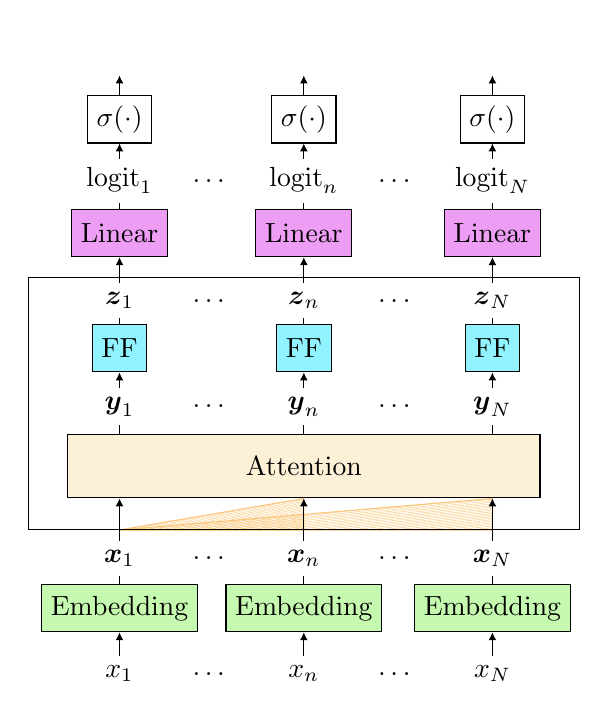
\begin{tikzpicture}[>={Latex[length=1mm,width=1mm]}, node distance=1.5cm]
        % x_i
        \node (x1) {$x_1$};
        \node[right=0.5cm of x1]    (dotsl_x) {$\dots$};
        \node[right=0.5cm of dotsl_x] (xn)    {$x_n$};
        \node[right=0.5cm of xn]    (dotsr_x) {$\dots$};
        \node[right=0.5cm of dotsr_x] (xN)    {$x_N$};
        %\node[right=-0.15cm of xN]       (set)  {$\in \{0,1\}$};
        % embed
        \foreach \i in {1,n,N}{
            \node[above=0.3cm of x\i, minimum height = 0.6cm] (embed\i) [draw, rectangle, fill=embed!70] {Embedding};
        }
        \node[above=1.6cm of x1] (x1-corner) {};
        \node[above=1.6cm of xn] (xn-corner) {};
        \node[above=1.6cm of xN] (xN-corner) {};
        % masked attention
        \node[above=2cm of xn, minimum width = 6cm, minimum height = 0.8cm] (attn) [draw, rectangle, fill=attn!50] {Attention};
        \fill[draw=attn!70!orange, pattern={Lines[angle=12, line width=0.2pt, distance=0.2mm]},pattern color=attn!80!orange] ([yshift=0cm]x1-corner.south) -- ([yshift=0cm]xn-corner.south) -- (attn.south -| embedn.north) -- ([yshift=0cm]x1-corner.south) -- cycle;
        \fill[draw=attn!70!orange, pattern={Lines[angle=6, line width=0.2pt, distance=0.2mm]},pattern color=attn!80!orange] ([yshift=0cm]x1-corner.south) -- ([yshift=0cm]xN-corner.south) -- (attn.south -| embedN.north) -- ([yshift=0cm]x1-corner.south) -- cycle;
        % big box containing everything
        \node[above=1.6cm of xn, minimum width = 7cm, minimum height = 3.2cm] (xfmr) [draw, rectangle] {};
        % arrows for \bx
        \foreach \i in {1,n,N}{
            \draw[->] (x\i) -- (x\i |- embed\i.south);
            \draw[->] (embed\i.north) -- (attn.south -| embed\i.north) node[pos=0.3,fill=white] (bx\i) {$\bx_{\i}$}; 
        }
        % dots for \bx
        \path (bx1) -- (bxn) node[midway] (midpoint) {$\dots$};
        \path (bxn) -- (bxN) node[midway] (midpoint) {$\dots$};
        % FF and arrows for \by
        \foreach \i in {1,n,N}{
            \node[above=3.6cm of x\i, minimum height = 0.6cm] (FF\i) [draw, rectangle, fill=ff] {FF};
            \draw[->] (attn.north -| FF\i.south) -- (FF\i.south) node[pos=0.45,fill=white] (by\i) {$\by_{\i}$}; 
        }
        % dots for \by
        \path (by1) -- (byn) node[midway] (midpoint) {$\dots$};
        \path (byn) -- (byN) node[midway] (midpoint) {$\dots$};
        % linear and arrows for \bz
        \foreach \i in {1,n,N}{
            \node[above=0.85cm of FF\i, minimum height = 0.6cm] (lin\i) [draw, rectangle, fill=lin!60] {Linear};
            \draw[->] (FF\i.north) -- (lin\i.south) node[pos=0.35,fill=white] (bz\i) {$\bz_{\i}$}; 
        }
        % dots for \bz
        \path (bz1) -- (bzn) node[midway] (midpoint) {$\dots$};
        \path (bzn) -- (bzN) node[midway] (midpoint) {$\dots$};
        % softmax and arrows for \logit
        \foreach \i in {1,n,N}{
            \node[above=0.83cm of lin\i, minimum height = 0.6cm] (soft\i) [draw, rectangle] {$\sigma(\cdot)$};
            \draw[->] (lin\i.north) -- (soft\i.south) node[pos=0.43,fill=white] (logit\i) {$\logit_{\i}$}; 
        }
        % dots for \logit
        \path (logit1) -- (logitn) node[midway] (midpoint) {$\dots$};
        \path (logitn) -- (logitN) node[midway] (midpoint) {$\dots$};
        % \bbP and arrows and dots
        % \node[above=0.4cm of soft1, minimum height = 0.6cm] (prob1) {\scalebox{0.8}{$\bbP_{\btheta}(x_{2} = 1 \mid x_1)$}};
        % \node[above=0.4cm of softn, minimum height = 0.6cm] (probn) {\scalebox{0.8}{$\bbP_{\btheta}(x_{n+1} = 1 \mid x_1^n)$}};
        % \node[above=0.4cm of softN, minimum height = 0.6cm] (probN) {\scalebox{0.8}{$\bbP_{\btheta}(x_{N+1} = 1 \mid x_1^N)$}};
        \foreach \i in {1,n,N}{
            \node[above=0.25cm of soft\i, minimum height = 0.6cm] (prob\i) {$$};
            \draw[->] (soft\i.north) -- (prob\i);
        }
      
        %\path (prob1) -- (probn) node[midway] (midpoint) {$\dots$};
        %\path (probn) -- (probN) node[midway] (midpoint) {$\dots$};
\end{tikzpicture}
\end{document}